\documentclass[12pt,a4paper]{article}

\usepackage[utf8]{inputenc}
\usepackage[T2A]{fontenc}
\usepackage[russian]{babel}
\usepackage{amsmath,amssymb,amsthm}
\usepackage{xcolor}
\usepackage{graphicx}
\usepackage{float}
\usepackage{booktabs}
\usepackage{array}
\usepackage{multirow}
\usepackage{geometry}
\geometry{left=2.5cm, right=2cm, top=2.5cm, bottom=2.5cm}
\usepackage[hidelinks]{hyperref}
\usepackage{fancyhdr}
\pagestyle{fancy}
\fancyhf{}
\fancyhead[L]{\small Вариант 14 (5130201/30102)}
\fancyhead[R]{\small Математическая статистика}
\fancyfoot[C]{\thepage}
\renewcommand{\headrulewidth}{0.4pt}

\usepackage{listings}
\lstset{
	language=R,
	basicstyle=\ttfamily\small,
	keywordstyle=\color{blue!70!black}\bfseries,
	commentstyle=\color{green!50!black}\itshape,
	numbers=left, numberstyle=\tiny\color{gray},
	frame=single, breaklines=true,
	showstringspaces=false,
	backgroundcolor=\color{gray!5},
	extendedchars=true, keepspaces=true
}

\newcommand{\lahat}{\hat{\lambda}}
\newcommand{\ahat}{\hat{a}}
\newcommand{\xbar}{\bar{x}}

\begin{document}
	
	%--- Титульная страница ---%
	\thispagestyle{empty}
	\begin{titlepage}
		\begin{center}
			\textbf{МИНИСТЕРСТВО НАУКИ И ВЫСШЕГО ОБРАЗОВАНИЯ\\
				РОССИЙСКОЙ ФЕДЕРАЦИИ}\\[6pt]
			Федеральное государственное автономное образовательное учреждение\\
			высшего образования <<Санкт-Петербургский политехнический\\
			университет Петра Великого>>\\[6pt]
			Институт компьютерных наук и кибербезопасности\\
			Высшая школа технологий искусственного интеллекта\\[6pt]
			Направление: 02.03.01 <<Математика и компьютерные науки>>
			
			\vfill
			
			{\large\textbf{Индивидуальное домашнее задание №3}}\\[6pt]
			по дисциплине\\[4pt]
			{\large <<Математическая статистика>>}\\[12pt]
			{\large Вариант №{} 14}
			
			\vfill
			
			\small{
				\begin{tabular}{lrrl}
					\!\!\!Студент, & \hspace{2cm} & & \\
					\!\!\!группы 5130201/30102 & \hspace{2cm} & \underline{\hspace{3cm}} & Санько В. В. \\\\
					\!\!\!Преподаватель & \hspace{2cm} & \underline{\hspace{3cm}} & Малов С. В. \\\\
					&&\hspace{4cm}
				\end{tabular}
				\begin{flushright}
					<<\underline{\hspace{1cm}}>>\underline{\hspace{2.5cm}} 2026 г.
				\end{flushright}
			}
			
			\hfill\break
			\begin{center}\small{Санкт-Петербург, 2026}\end{center}
		\end{center}
	\end{titlepage}
	
	\tableofcontents
	\newpage
	
	%=============================================================
	\section{Часть 1. Распределение Пуассона}
	%=============================================================
	
	\subsection{Исходные данные}
	
	\[
	\alpha_1 = 0{,}05;\quad a = 0{,}00;\quad b = 1{,}20;\quad
	\lambda_0 = 1{,}40;\quad \lambda_1 = 0{,}70.
	\]
	
	\begin{table}[H]
		\centering
		\begin{tabular}{|c|c|c|c|c|c|c|c|c|c|}
			\hline
			1&0&1&1&3&1&0&1&0&1\\
			\hline
			1&1&0&1&1&0&0&1&2&0\\
			\hline
			1&1&0&1&1&0&2&0&0&0\\
			\hline
			0&1&1&0&0&2&0&1&0&1\\
			\hline
			1&0&1&0&0&0&1&2&0&2\\
			\hline
		\end{tabular}
		\caption{Данные эксперимента ($n=50$)}
	\end{table}
	
	%-------------------------------------------------------------
	\subsection{a) Вариационный ряд, ECDF и гистограмма}
	
	\textbf{Задание:} построить вариационный ряд, эмпирическую функцию распределения
	и гистограмму частот.
	
	\textbf{Вариационный ряд} (упорядоченный набор исходных данных):
	
	\begin{table}[H]
		\centering
		\begin{tabular}{|c|c|c|c|c|c|c|c|c|c|}
			\hline
			0&0&0&0&0&0&0&0&0&0\\
			\hline
			0&0&0&0&0&0&0&0&0&0\\
			\hline
			0&0&1&1&1&1&1&1&1&1\\
			\hline
			1&1&1&1&1&1&1&1&1&1\\
			\hline
			1&1&1&1&2&2&2&2&2&3\\
			\hline
		\end{tabular}
		\caption{Вариационный ряд}
	\end{table}
	
	\textbf{Эмпирическая функция распределения} показывает долю элементов выборки $\le x$:
	\[
	F^*(x) = \frac{1}{n}\sum_{i=1}^{n}\mathbf{1}[x_i \le x].
	\]
	
	\begin{table}[H]
		\centering
		\begin{tabular}{ccccc}
			\toprule
			$x_i$ & $n_i$ & $\tilde{n}_i = n_i/n$ & $F^*(x_i)$ \\
			\midrule
			0 & 22 & 0{,}44 & 0{,}44 \\
			1 & 22 & 0{,}44 & 0{,}88 \\
			2 &  5 & 0{,}10 & 0{,}98 \\
			3 &  1 & 0{,}02 & 1{,}00 \\
			\bottomrule
		\end{tabular}
		\caption{Таблица частот}
	\end{table}
	
Графики ECDF и гистограммы строятся в R:
\begin{lstlisting}
	plot(ecdf(x), main="Empirical CDF", xlab="x", ylab="F*(x)")
	barplot(table(x)/length(x), main="Frequency histogram")
\end{lstlisting}

\begin{figure}[H]
	\centering
	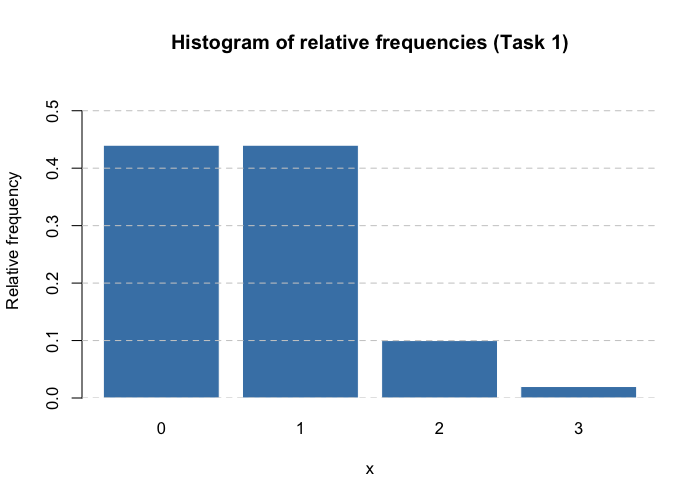
\includegraphics[width=0.48\textwidth]{plots/task1_histogram}
	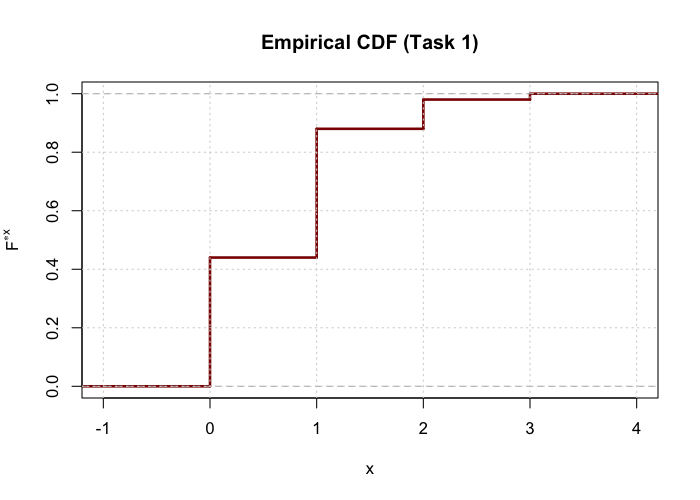
\includegraphics[width=0.48\textwidth]{plots/task1_ecdf}
	\caption{Задание 1: Гистограмма относительных частот (слева) и эмпирическая функция распределения (справа)}
\end{figure}
	
	%-------------------------------------------------------------
	\subsection{b) Числовые характеристики выборки}
	
	\textbf{Задание:} вычислить выборочные аналоги числовых характеристик:
	математического ожидания, дисперсии, медианы, асимметрии, эксцесса,
	вероятности $P(X \in [a, b])$.
	
	\begin{enumerate}
		\item \textbf{Математическое ожидание:}
		\[
		\xbar = \frac{1}{n}\sum_{i=1}^n x_i
		= \frac{0\cdot22 + 1\cdot22 + 2\cdot5 + 3\cdot1}{50} = \frac{35}{50} = 0{,}70.
		\]
		
		\item \textbf{Дисперсия:}
		\[
		s^2 = \frac{1}{n-1}\sum_{i=1}^n(x_i-\xbar)^2 = 0{,}5408.
		\]
		
		\item \textbf{Медиана:}
		\[
		\mathrm{Me} = \frac{x_{(25)}+x_{(26)}}{2} = \frac{1+1}{2} = 1{,}00.
		\]
		
		\item \textbf{Асимметрия:}
		\[
		A_s = \frac{\mu_3}{\mu_2^{3/2}} = \frac{\frac{1}{n}\sum(x_i-\xbar)^3}
		{\left(\frac{1}{n}\sum(x_i-\xbar)^2\right)^{3/2}} = 0{,}8397
		\]
		(правосторонняя: больше значений сосредоточено слева от среднего).
		
		\item \textbf{Эксцесс:}
		\[
		E_x = \frac{\mu_4}{\mu_2^2} - 3 = 0{,}3980.
		\]
		
		\item \textbf{Вероятность:}
		\[
		P^*(X \in [a,b]) = P^*(X \in [0{,}00;\,1{,}20])
		= \frac{|\{x_i : 0 \le x_i \le 1{,}2\}|}{50} = \frac{44}{50} = 0{,}88.
		\]
	\end{enumerate}
	
	\textbf{Ответ:} $\xbar = 0{,}70$;\; $s^2 = 0{,}5408$;\;
	$\mathrm{Me} = 1{,}00$;\; $A_s = 0{,}84$;\; $E_x = 0{,}40$;\;
	$P^* = 0{,}88$.
	
	%-------------------------------------------------------------
	\subsection{c) Оценки параметра \texorpdfstring{$\lambda$}{lambda}}
	
	\textbf{Задание:} построить оценку МПП и оценку по методу моментов
	параметра $\lambda$. Найти смещения оценок.
	
	Распределение Пуассона:
	\[
	P_\lambda(X=k) = \frac{\lambda^k e^{-\lambda}}{k!},\quad k=0,1,2,\ldots
	\]
	
	\subsubsection*{Оценка максимального правдоподобия}
	
	Функция правдоподобия:
	\[
	L(x,\lambda) = \prod_{i=1}^n \frac{\lambda^{x_i}e^{-\lambda}}{x_i!}.
	\]
	Логарифм:
	\[
	LL(x,\lambda) = \sum_{i=1}^n x_i\ln\lambda - n\lambda - \sum_{i=1}^n\ln(x_i!).
	\]
	Берём производную и приравниваем к нулю:
	\[
	\frac{\partial LL}{\partial\lambda} = \frac{1}{\lambda}\sum_{i=1}^n x_i - n = 0
	\quad\Rightarrow\quad
	\lahat_{\text{МПП}} = \frac{1}{n}\sum_{i=1}^n x_i = \xbar.
	\]
	
	\subsubsection*{Оценка по методу моментов}
	
	Теоретический 1-й момент: $EX = \lambda$. Выборочный первый момент: $\xbar$.
	Приравниваем: $\lambda = \xbar$ --- совпадает с МПП.
	
	\subsubsection*{Смещение}
	
	Для обеих оценок:
	\[
	E\xbar = E\!\left(\frac{1}{n}\sum_{i=1}^n x_i\right)
	= \frac{1}{n}\sum_{i=1}^n EX_i = \frac{1}{n}\cdot n\lambda = \lambda,
	\quad E\xbar - \lambda = 0.
	\]
	$\Rightarrow$ оценка \textbf{несмещённая}.
	
	\textbf{Ответ:} МПП $= \lahat = 0{,}70$;\; ММ $= 0{,}70$;\; смещение $= 0$.
	
	%-------------------------------------------------------------
	\subsection{d) Доверительный интервал для \texorpdfstring{$\lambda$}{lambda}}
	
	\textbf{Задание:} построить асимптотический доверительный интервал уровня
	значимости $\alpha_1$ для $\lambda$ на базе МПП.
	
	Уровень значимости $\alpha_1 = 0{,}05$, уровень доверия $1-\alpha_1 = 0{,}95$.
	
	По информации Фишера для Пуассона $I(\lambda) = 1/\lambda$, поэтому:
	\[
	\sqrt{n}(\lahat-\lambda) \xrightarrow{d} N(0,\lambda).
	\]
	Из состоятельности оценки делаем замену $\lambda$ на $\lahat$:
	\[
	\frac{\sqrt{n}(\lahat-\lambda)}{\sqrt{\lahat}} \xrightarrow{d} N(0,1).
	\]
	Доверительный интервал:
	\[
	\lambda \in \left[\lahat - z_{\alpha_1/2}\cdot\sqrt{\frac{\lahat}{n}}\,;\;
	\lahat + z_{\alpha_1/2}\cdot\sqrt{\frac{\lahat}{n}}\right].
	\]
	
	Числовые значения:
	\begin{itemize}
		\item $z_{\alpha_1/2} = z_{0{,}025} = 1{,}96$ --- квантиль нормального распределения,
		\item $\sqrt{\lahat/n} = \sqrt{0{,}70/50} = 0{,}1183$ --- стандартная ошибка,
		\item $\lahat - z_{\alpha_1/2}\cdot\sqrt{\lahat/n} = 0{,}70 - 1{,}96\cdot0{,}1183 = 0{,}4681$ --- левая граница,
		\item $\lahat + z_{\alpha_1/2}\cdot\sqrt{\lahat/n} = 0{,}70 + 1{,}96\cdot0{,}1183 = 0{,}9319$ --- правая граница.
	\end{itemize}
	
	\textbf{Ответ:} $\lambda \in [0{,}4681;\; 0{,}9319]$ с уровнем доверия $0{,}95$.
	
	%-------------------------------------------------------------
	\subsection{e) Критерий \texorpdfstring{$\chi^2$}{chi2}: простая гипотеза
		\texorpdfstring{$H_0\colon\mathrm{Poisson}(\lambda_0)$}{}}
	
	\textbf{Задание:} используя гистограмму частот, построить критерий $\chi^2$
	проверки простой гипотезы согласия с распределением Пуассона с параметром $\lambda_0$.
	Проверить гипотезу на уровне значимости $\alpha_1$.
	
	\subsubsection*{Описание процедуры проверки гипотезы}
	
	Проверяем гипотезу $H_0$: выборка подчиняется распределению Пуассона
	с параметром $\lambda = \lambda_0 = 1{,}40$, против альтернативы $H_A$:
	выборка не подчиняется указанному распределению.
	
	\begin{enumerate}
		\item \textbf{Разбиение на интервалы.}
		Выбираем границы интервалов так, чтобы в каждом было не менее 5 наблюдений.
		Объединяем хвост $X \ge 3$:
		
		\begin{table}[H]
			\centering
			\begin{tabular}{ccc}
				\toprule
				$i$ & range & $\nu_i$ \\
				\midrule
				1 & $X = 0$   & 22 \\
				2 & $X = 1$   & 22 \\
				3 & $X \ge 2$ &  6 \\
				\bottomrule
			\end{tabular}
			\caption{Диапазоны и количество наблюдений}
		\end{table}
		
		\item \textbf{Наблюдаемые частоты:} $\nu_j = \sum_{i=1}^n \mathbf{1}\{X_i \in I_j\}$.
		
		\item \textbf{Теоретические вероятности} при $\lambda_0 = 1{,}40$:
		\[
		p_1 = P(X=0) = e^{-1{,}4} = 0{,}2466,\quad
		p_2 = P(X=1) = 1{,}4e^{-1{,}4} = 0{,}3452,
		\]
		\[
		p_3 = P(X\ge2) = 1 - P(X\le1) = 0{,}4082.
		\]
		
		\item \textbf{Ожидаемые частоты:} $E_j = n\cdot p_j$.
		
		\item \textbf{Статистика критерия:}
		\[
		\chi^2 = \sum_{j=1}^k \frac{(\nu_j - E_j)^2}{E_j}.
		\]
		
		\item \textbf{Критическая область:} $\chi^2 > \chi^2_{1-\alpha_1}(k-1)$,
		где $k$ --- число интервалов, $r=0$ --- число оцениваемых параметров.
		
		\item \textbf{Принятие решения:} если $\chi^2 \le \chi^2_{1-\alpha_1}(k-r-1)$,
		$H_0$ не отвергается.
		
		\item \textbf{P-значение:} $p = 1 - F_{\chi^2}(\chi^2;\,k-r-1)$.
	\end{enumerate}
	
	\subsubsection*{Результаты вычислений}
	
	\begin{table}[H]
		\centering
		\begin{tabular}{ccccccc}
			\toprule
			$i$ & range & $\nu_i$ & $p_i$ & $np_i$ &
			$\mathrm{res} = \frac{\nu_i - np_i}{\sqrt{np_i}}$ & $\mathrm{res}^2$ \\
			\midrule
			1 & $X=0$    & 22 & 0{,}2466 & 12{,}330 & $+2{,}754$ &  7{,}584 \\
			2 & $X=1$    & 22 & 0{,}3452 & 17{,}262 & $+1{,}140$ &  1{,}301 \\
			3 & $X\ge2$  &  6 & 0{,}4082 & 20{,}408 & $-3{,}189$ & 10{,}172 \\
			\bottomrule
			\multicolumn{6}{r}{$\chi^2 =$} & \textbf{16{,}879} \\
		\end{tabular}
		\caption{Сводная таблица для проверки гипотезы $H_0\colon\mathrm{Poisson}(1{,}4)$}
	\end{table}
	
	\begin{enumerate}
		\item \textbf{Степени свободы:} $df = k - 1 = 3 - 1 = 2$.
		\item \textbf{Статистика $\chi^2$:} $\chi^2 = 19{,}057$.
		\item \textbf{Критическое значение:} $\mathrm{crit} = \chi^2_{0{,}95}(2) = 5{,}991$.
		\item \textbf{P-значение:} $p = 0{,}0001$.
	\end{enumerate}
	
	Поскольку $\chi^2 = 19{,}057 > 5{,}991 = \mathrm{crit}$, нулевая гипотеза $H_0$ \textbf{отвергается}.
	Данные нельзя считать подчиняющимися распределению Пуассона с параметром $\lambda_0 = 1{,}40$.
	
	\textbf{Наибольший уровень значимости, на котором $H_0$ не отвергается}:
	$p\text{-значение} = 0{,}0001$.
	
	\begin{figure}[H]
		\centering
		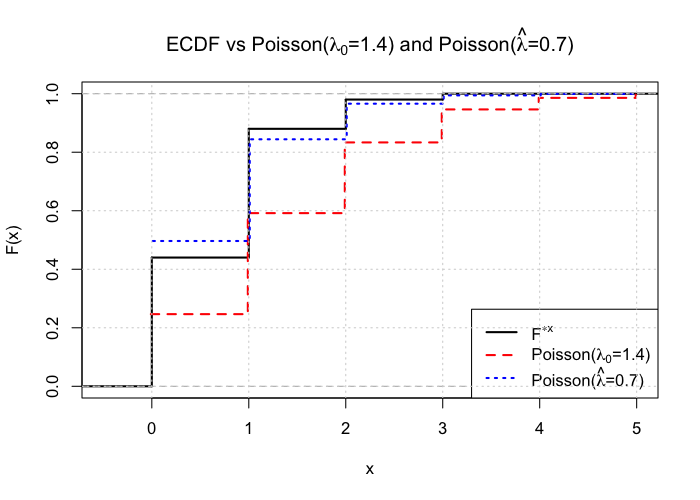
\includegraphics[width=0.7\textwidth]{plots/task1_ecdf_vs_theor}
		\caption{Задание 1: ECDF vs теоретические Poisson($\lambda_0=1{,}4$) и Poisson($\hat\lambda=0{,}7$)}
	\end{figure}
	
	%-------------------------------------------------------------
	\subsection{f) Критерий \texorpdfstring{$\chi^2$}{chi2}: сложная гипотеза
		\texorpdfstring{$H_0\colon\mathrm{Poisson}(\lambda)$}{}}
	
	\textbf{Задание:} построить критерий $\chi^2$ проверки сложной гипотезы согласия
	с распределением Пуассона. Проверить гипотезу на уровне значимости $\alpha_1$.
	
	\subsubsection*{Постановка задачи}
	
	Нулевая гипотеза $H_0$: данные выборки следуют распределению Пуассона
	с параметром $\lambda > 0$.
	
	Сложная гипотеза --- нам не дано $\lambda_0$. Оцениваем $\lambda$ путём
	минимизации статистики $\chi^2$ по группированным данным:
	\[
	\chi^2(\lambda) = \sum_{j=1}^k \frac{(\nu_j - np_j(\lambda))^2}{np_j(\lambda)},
	\]
	где $p_j(\lambda)$ --- теоретические вероятности попадания в интервал $I_j$.
	
	Минимизация выполняется в R через \texttt{nlm(csq.stat, lambda\_mle)}.
	Оптимальное значение: $\hat\lambda_{\chi^2} = 0,7233$
	(не совпадает с $\bar{x} = 0,70$, оценивается по группированным данным).
	
	\subsubsection*{Вычисление теоретических вероятностей}
	
	\[
	p_1(\lambda) = P(X=0) = e^{-\lambda},\quad
	p_2(\lambda) = P(X=1) = \lambda e^{-\lambda},
	\]
	\[
	p_3(\lambda) = P(X\ge2) = 1 - P(X\le1)
	\]
	
	\subsubsection*{Результаты вычислений}
	
	\begin{table}[H]
		\centering
		\begin{tabular}{ccccccc}
			\toprule
			$i$ & range & $\nu_i$ & $p_i(\hat\lambda)$ & $np_i$ &
			$\mathrm{res}$ & $\mathrm{res}^2$ \\
			\midrule
			1 & $X=0$    & 22 & 0{,}4851 & 24{,}257 & $-0{,}458$ & 0{,}210 \\
			2 & $X=1$    & 22 & 0{,}3509 & 17{,}545 & $+1{,}063$ & 1{,}131 \\
			3 & $X\ge2$  &  6 & 0{,}1639 &  8{,}197 & $-0{,}767$ & 0{,}589 \\
			\bottomrule
			\multicolumn{6}{r}{$\chi^2_{\min} =$} & \textbf{1{,}930} \\
		\end{tabular}
		\caption{Сводная таблица для сложной гипотезы $\mathrm{Poisson}(\hat\lambda_{\chi^2})$}
	\end{table}
	
	\begin{enumerate}
		\item \textbf{Степени свободы:} $df = k - 1 - p = 3 - 1 - 1 = 1$
		($p=1$ --- число оцениваемых параметров).
		\item \textbf{Статистика $\chi^2$:} $\chi^2 = 1{,}930$.
		\item \textbf{Критическое значение:} $\mathrm{crit} = \chi^2_{0{,}95}(1) = 3{,}841$.
		\item \textbf{P-значение:} $p = 0{,}165$.
	\end{enumerate}
	
	Поскольку $\chi^2 = 1{,}930 < 3{,}841 = \mathrm{crit}$, нулевая гипотеза $H_0$
	\textbf{не отвергается}. Данные совместимы с распределением Пуассона.
	
	\textbf{Наибольший уровень значимости}: $p\text{-значение} = 0{,}165$.
	
	\begin{figure}[H]
		\centering
		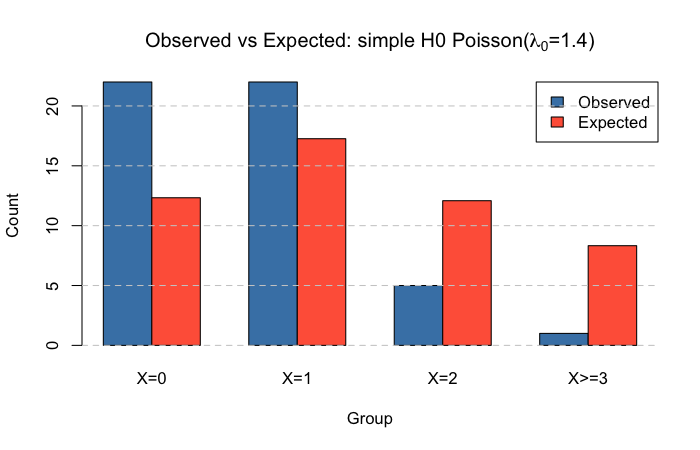
\includegraphics[width=0.48\textwidth]{plots/task1_chi2_simple}
		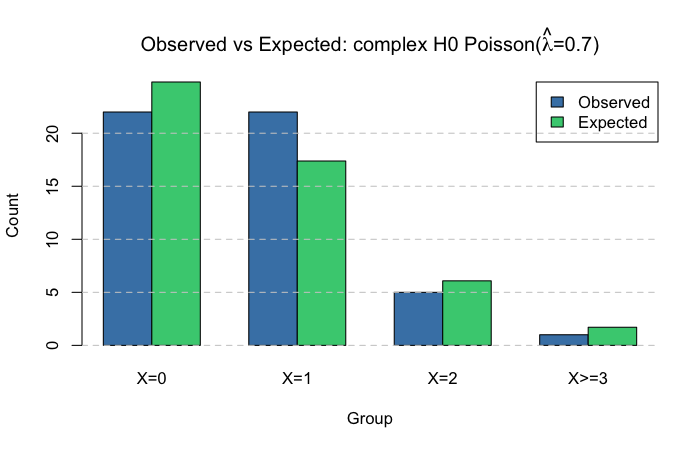
\includegraphics[width=0.48\textwidth]{plots/task1_chi2_complex}
		\caption{Задание 1: Наблюдаемые и ожидаемые частоты --- простая $H_0$ (слева) и сложная $H_0$ (справа)}
	\end{figure}
	
	%-------------------------------------------------------------
	\subsection{g) Наиболее мощный критерий (НМК)}
	
	\textbf{Задание:} построить наиболее мощный критерий проверки простой гипотезы
	пуассоновости с параметром $\lambda = \lambda_0$ при альтернативе с параметром
	$\lambda = \lambda_1$. Что получится, если поменять местами основную и
	альтернативную гипотезы?
	
	\subsubsection*{Постановка задачи}
	
	Нулевая гипотеза $H_0\colon \lambda = \lambda_0 = 1{,}40$,
	альтернативная $H_A\colon \lambda = \lambda_1 = 0{,}70$,
	уровень значимости $\alpha_1 = 0{,}05$.
	
	\subsubsection*{Функция правдоподобия}
	
	\[
	L(x;\lambda) = \prod_{i=1}^n \frac{\lambda^{x_i}e^{-\lambda}}{x_i!}.
	\]
	
	Согласно лемме Неймана--Пирсона, наиболее мощный критерий основан на
	отношении правдоподобия:
	\[
	LR(X) = \frac{L(X;\lambda_1)}{L(X;\lambda_0)}
	= \left(\frac{\lambda_1}{\lambda_0}\right)^{\sum x_i}
	e^{n(\lambda_0-\lambda_1)}.
	\]
	
	\subsubsection*{Переход к логарифму}
	
	\[
	\ln LR(X) = n(\lambda_0-\lambda_1) + \left(\sum_{i=1}^n X_i\right)\ln\frac{\lambda_1}{\lambda_0}.
	\]
	
	При $\lambda_1 < \lambda_0$ имеем $\ln(\lambda_1/\lambda_0) < 0$, то есть
	$\ln LR(X)$ \textbf{убывает} с ростом $\sum X_i$. Критическая область:
	\[
	\sum_{i=1}^n X_i \le C,
	\]
	где $C$ находится из условия $P_{H_0}\!\left(\sum X_i \le C\right) \le \alpha_1$.
	
	\subsubsection*{Нахождение границы $C$}
	
	При $H_0$ сумма наблюдений распределена как:
	\[
	S = \sum_{i=1}^n X_i \sim \mathrm{Poisson}(n\lambda_0) = \mathrm{Poisson}(70).
	\]
	
	Используем функцию \texttt{qpois} в R:
	\[
	C \leftarrow \texttt{qpois}(\alpha_1,\, n\lambda_0).
	\]
	
	Для $\alpha_1 = 0{,}05$ и $n\lambda_0 = 70$:
	\begin{itemize}
		\item $P(S \le 57 \mid H_0) \approx 0{,}0641$,
		\item $P(S \le 56 \mid H_0) \approx 0{,}0451 < 0{,}05$.
	\end{itemize}
	Следовательно, $C = 57$.
	
	\subsubsection*{Формальная запись критерия через $\phi(X)$}
	
	\[
	\phi(X) = \begin{cases}
		1, & \text{если } \sum_{i=1}^n X_i < 57,\\
		p, & \text{если } \sum_{i=1}^n X_i = 57,\\
		0, & \text{если } \sum_{i=1}^n X_i > 57,
	\end{cases}
	\]
	где $p$ определяется из условия:
	\[
	P_{H_0}\!\left(\sum X_i < 57\right) + p\cdot P_{H_0}\!\left(\sum X_i = 57\right) = \alpha_1.
	\]
	\[
	p = \frac{0{,}05 - 0{,}0451}{0{,}0641 - 0{,}0451} \approx 0{,}258.
	\]
	
	\subsubsection*{Проверка гипотезы}
	
	Наблюдаемое значение: $\sum_{i=1}^n X_i = 35 < 57 = C$.
	
	$\Rightarrow$ гипотеза $H_0$ \textbf{отвергается}.
	
	\textbf{Мощность критерия:}
	\[
	\beta = P\!\left(\sum X_i \le 57 \mid H_1\right) = F_{\mathrm{Poisson}(35)}(57) \approx 0{,}9998.
	\]
	
	\begin{figure}[H]
		\centering
		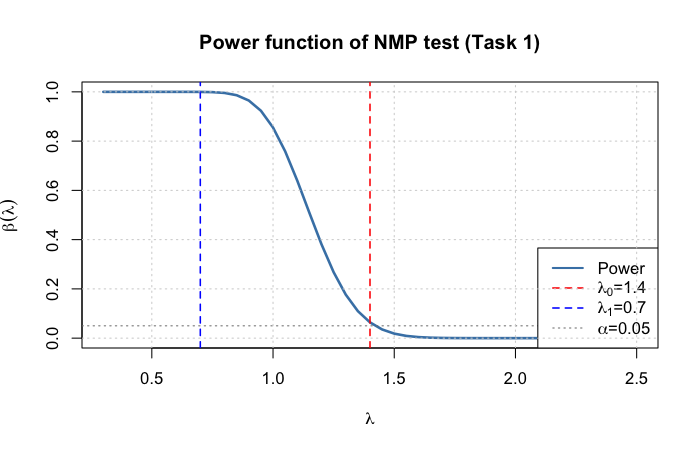
\includegraphics[width=0.7\textwidth]{plots/task1_nmk_power}
		\caption{Задание 1: Функция мощности $\beta(\lambda)$ наиболее мощного критерия, $C=57$}
	\end{figure}
	
	\subsubsection*{Смена гипотез местами}
	
	Нулевая гипотеза: $H_0\colon\lambda = \lambda_1 = 0{,}70$,
	альтернатива: $H_A\colon\lambda = \lambda_0 = 1{,}40$.
	
	Теперь $\ln LR(X)$ \textbf{возрастает} с ростом $\sum X_i$,
	критическая область \textbf{правосторонняя}: $\sum X_i \ge C'$.
	
	При $H_0$: $S \sim \mathrm{Poisson}(35)$.
	$C' \leftarrow \texttt{qpois}(1-\alpha_1,\, n\lambda_1) = 45$.
	
	\[
	\phi(X) = \begin{cases}
		1, & \text{если } \sum X_i > 45,\\
		p, & \text{если } \sum X_i = 45,\\
		0, & \text{если } \sum X_i < 45,
	\end{cases}
	\quad p \approx 0{,}188.
	\]
	
	При наблюдаемом значении $\sum X_i = 35 < 45 = C'$, гипотеза $H_0$
	\textbf{не отвергается}.
	
	%-------------------------------------------------------------
	\subsection{h) Геометрическое распределение}
	
	\textbf{Задание:} в пунктах (c)--(g) заменить семейство распределений Пуассона
	на семейство геометрических распределений:
	\[
	P_\lambda(X=k) = \frac{\lambda^k}{(\lambda+1)^{k+1}},\quad k=0,1,2,\ldots,\quad
	E[X]=\lambda.
	\]
	
	\subsubsection*{(c) Оценки}
	МПП и ММ совпадают: $\lahat = \xbar = 0{,}70$ (несмещённая оценка).
	
	\subsubsection*{(d) Доверительный интервал}
	$D[X] = \lambda(\lambda+1)$, по ЦПТ:
	\[
	\lahat \pm z_{0{,}975}\sqrt{\frac{\lahat(\lahat+1)}{n}}
	= 0{,}70 \pm 1{,}96\sqrt{\frac{1{,}19}{50}}
	= 0{,}70 \pm 0{,}3024.
	\]
	\[
	\lambda \in [0{,}398;\; 1{,}002].
	\]
	
	\subsubsection*{(e) $\chi^2$ простая гипотеза $H_0\colon\mathrm{Geom}(\lambda_0=1{,}4)$}
	
	\begin{table}[H]
		\centering
		\begin{tabular}{cccccc}
			\toprule
			$i$ & range & $\nu_i$ & $np_i$ & $\mathrm{res}$ & $\mathrm{res}^2$ \\
			\midrule
			1 & $X=0$   & 22 & 20{,}833 & $+0{,}256$ &  0{,}065 \\
			2 & $X=1$   & 22 & 12{,}153 & $+2{,}825$ &  7{,}979 \\
			3 & $X\ge2$ &  6 & 17{,}014 & $-2{,}670$ &  7{,}130 \\
			\bottomrule
			\multicolumn{5}{r}{$\chi^2 =$} & \textbf{15{,}174} \\
		\end{tabular}
		\caption{Геометрическое распределение: простая гипотеза}
	\end{table}
	
	$df=2$, $\mathrm{crit}=5{,}991$, $p=0{,}0005$. $H_0$ \textbf{отвергается}.
	
	\subsubsection*{(f) $\chi^2$ сложная гипотеза $H_0\colon\mathrm{Geom}(\hat\lambda_{\chi^2})$}
	
	Оцениваем $\lambda$ минимизацией $\chi^2$ по группированным данным:
	$\hat\lambda_{\chi^2} = 0{,}8158$ (не совпадает с $\bar{x}=0{,}70$).
	
	\begin{table}[H]
		\centering
		\begin{tabular}{cccccc}
			\toprule
			$i$ & range & $\nu_i$ & $np_i(\hat\lambda_{\chi^2})$ & $\mathrm{res}$ & $\mathrm{res}^2$ \\
			\midrule
			1 & $X=0$   & 22 & 27{,}536 & $-1{,}055$ &  1{,}113 \\
			2 & $X=1$   & 22 & 12{,}371 & $+2{,}738$ &  7{,}494 \\
			3 & $X\ge2$ &  6 & 10{,}093 & $-1{,}288$ &  1{,}660 \\
			\bottomrule
			\multicolumn{5}{r}{$\chi^2_{\min} =$} & \textbf{10{,}267} \\
		\end{tabular}
		\caption{Геометрическое распределение: сложная гипотеза}
	\end{table}
	
	$df=1$, $\mathrm{crit}=3{,}841$, $p=0{,}0014$. $H_0$ \textbf{отвергается}.
	
	\subsubsection*{(g) НМК для геометрического}
	
	$T = \sum x_i$ --- достаточная статистика.
	$E[T|H_0]=n\lambda_0=70$, $D[T|H_0]=n\lambda_0(\lambda_0+1)=168$.
	По ЦПТ: $c = 48$, $T_{\text{набл}}=35 \le 48$, $H_0$ \textbf{отвергается}.
	
	\newpage
	%=============================================================
	\section{Часть 2. Нормальное распределение}
	%=============================================================
	
	\subsection{Исходные данные}
	
	\[
	\alpha_2 = 0{,}10;\quad c = 2{,}60;\quad d = 4{,}60;\quad h = 0{,}80;\quad
	a_0 = 9{,}00;\quad \sigma_0 = 2{,}00;\quad a_1 = 3{,}00;\quad \sigma_1 = 2{,}00.
	\]
	
	\begin{table}[H]
		\centering
		\small
		\begin{tabular}{|c|c|c|c|c|c|c|c|c|c|}
			\hline
			8{,}752&2{,}202&2{,}779&2{,}717&2{,}033&2{,}755&3{,}688&4{,}318&2{,}188&2{,}878\\
			\hline
			2{,}243&3{,}204&3{,}076&4{,}700&2{,}244&4{,}634&3{,}069&1{,}574&5{,}394&4{,}323\\
			\hline
			2{,}691&1{,}079&2{,}726&1{,}260&$-$3{,}224&3{,}050&3{,}714&4{,}449&2{,}096&3{,}271\\
			\hline
			3{,}834&1{,}621&3{,}466&3{,}764&2{,}349&$-$1{,}848&4{,}301&1{,}119&0{,}639&7{,}699\\
			\hline
			4{,}572&3{,}146&2{,}898&3{,}383&3{,}535&3{,}054&6{,}165&4{,}822&2{,}797&$-$0{,}056\\
			\hline
		\end{tabular}
		\caption{Данные эксперимента ($n=50$)}
	\end{table}
	
	%-------------------------------------------------------------
	\subsection{a) Вариационный ряд, ECDF, гистограмма и полигон частот}
	
	\textbf{Задание:} построить вариационный ряд, эмпирическую функцию распределения,
	гистограмму и полигон частот с шагом $h$.
	
	\begin{table}[H]
		\centering
		\small
		\begin{tabular}{ccccc}
			\toprule
			Интервал & Середина $t_j$ & $n_j$ & $\tilde{n}_j$ & $F^*(t_j)$ \\
			\midrule
			$[-4{,}0;\;-3{,}2)$ & $-3{,}6$ &  1 & 0{,}02 & 0{,}02 \\
			$[-3{,}2;\;-2{,}4)$ & $-2{,}8$ &  0 & 0{,}00 & 0{,}02 \\
			$[-2{,}4;\;-1{,}6)$ & $-2{,}0$ &  1 & 0{,}02 & 0{,}04 \\
			$[-1{,}6;\;-0{,}8)$ & $-1{,}2$ &  0 & 0{,}00 & 0{,}04 \\
			$[-0{,}8;\;\phantom{-}0{,}0)$ & $-0{,}4$ & 1 & 0{,}02 & 0{,}06 \\
			$[\phantom{-}0{,}0;\;\phantom{-}0{,}8)$ & $0{,}4$ & 1 & 0{,}02 & 0{,}08 \\
			$[\phantom{-}0{,}8;\;\phantom{-}1{,}6)$ & $1{,}2$ & 4 & 0{,}08 & 0{,}16 \\
			$[\phantom{-}1{,}6;\;\phantom{-}2{,}4)$ & $2{,}0$ & 8 & 0{,}16 & 0{,}32 \\
			$[\phantom{-}2{,}4;\;\phantom{-}3{,}2)$ & $2{,}8$ & 13 & 0{,}26 & 0{,}58 \\
			$[\phantom{-}3{,}2;\;\phantom{-}4{,}0)$ & $3{,}6$ & 9 & 0{,}18 & 0{,}76 \\
			$[\phantom{-}4{,}0;\;\phantom{-}4{,}8)$ & $4{,}4$ & 7 & 0{,}14 & 0{,}90 \\
			$[\phantom{-}4{,}8;\;\phantom{-}5{,}6)$ & $5{,}2$ & 2 & 0{,}04 & 0{,}94 \\
			$[\phantom{-}5{,}6;\;\phantom{-}6{,}4)$ & $6{,}0$ & 1 & 0{,}02 & 0{,}96 \\
			$[\phantom{-}6{,}4;\;\phantom{-}7{,}2)$ & $6{,}8$ & 0 & 0{,}00 & 0{,}96 \\
			$[\phantom{-}7{,}2;\;\phantom{-}8{,}0)$ & $7{,}6$ & 1 & 0{,}02 & 0{,}98 \\
			$[\phantom{-}8{,}0;\;\phantom{-}8{,}8]$ & $8{,}4$ & 1 & 0{,}02 & 1{,}00 \\
			\bottomrule
		\end{tabular}
		\caption{Интервальная таблица частот (шаг $h=0{,}80$)}
	\end{table}
	
	\begin{figure}[H]
		\centering
		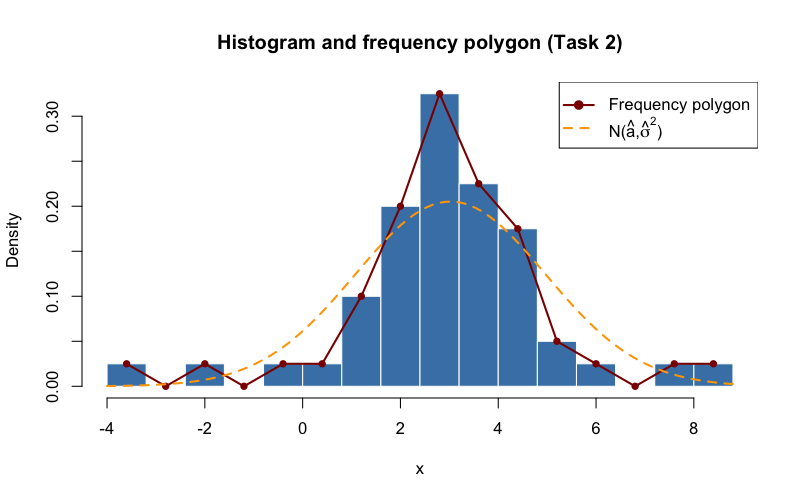
\includegraphics[width=0.48\textwidth]{plots/task2_histogram}
		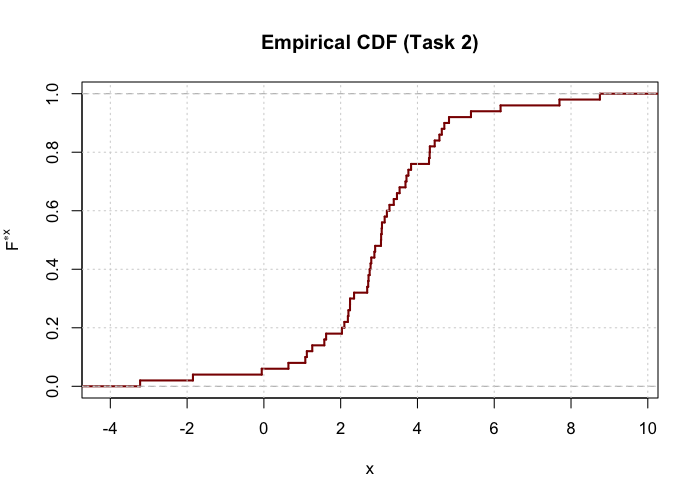
\includegraphics[width=0.48\textwidth]{plots/task2_ecdf}
		\caption{Задание 2: Гистограмма с полигоном частот (слева) и эмпирическая функция распределения (справа)}
	\end{figure}
	
	%-------------------------------------------------------------
	\subsection{b) Числовые характеристики выборки}
	
	\textbf{Задание:} вычислить выборочные аналоги числовых характеристик.
	
	\begin{enumerate}
		\item \textbf{Математическое ожидание:}
		\[
		\xbar = \frac{1}{n}\sum_{i=1}^n x_i = \frac{151{,}145}{50} = 3{,}0229.
		\]
		
		\item \textbf{Дисперсия:}
		\[
		s^2 = \frac{1}{n-1}\sum_{i=1}^n(x_i-\xbar)^2 = 3{,}8566,\qquad
		D = \frac{n-1}{n}s^2 = 3{,}7794.
		\]
		
		\item \textbf{Медиана:}
		\[
		\mathrm{Me} = \frac{x_{(25)}+x_{(26)}}{2} = \frac{3{,}050+3{,}054}{2} = 3{,}052.
		\]
		
		\item \textbf{Асимметрия:}
		\[
		A_s = \frac{\mu_3}{\mu_2^{3/2}} = -0{,}1839
		\]
		(левосторонняя: значения сосредоточены справа от среднего).
		
		\item \textbf{Эксцесс:}
		\[
		E_x = \frac{\mu_4}{\mu_2^2} - 3 = 2{,}581
		\]
		(островершинное распределение).
		
		\item \textbf{Вероятность:}
		\[
		P^*(X \in [c,d]) = P^*(X \in [2{,}6;\,4{,}6])
		= \frac{27}{50} = 0{,}54.
		\]
	\end{enumerate}
	
	\textbf{Ответ:} $\xbar=3{,}023$;\; $s^2=3{,}857$;\; $\mathrm{Me}=3{,}052$;\;
	$A_s=-0{,}184$;\; $E_x=2{,}581$;\; $P^*=0{,}54$.
	
	%-------------------------------------------------------------
	\subsection{c) Оценки параметров нормального распределения}
	
	\textbf{Задание:} построить оценку МПП параметров $(a,\sigma^2)$ и оценки по
	методу моментов. Найти смещения оценок.
	
	\[
	f(x) = \frac{1}{\sqrt{2\pi}\sigma}\exp\!\left(-\frac{(x-a)^2}{2\sigma^2}\right).
	\]
	
	\subsubsection*{Оценки максимального правдоподобия}
	
	\[
	LL(X;a,\sigma^2) = -\frac{n}{2}\log(2\pi) - \frac{n}{2}\log(\sigma^2)
	- \frac{1}{2\sigma^2}\sum_{i=1}^n(X_i-a)^2.
	\]
	
	Для нахождения оценок берём производные по $a$ и $\sigma^2$,
	приравниваем к нулю:
	\[
	\ahat = \xbar = 3{,}0229,\qquad
	\hat\sigma^2 = \frac{1}{n}\sum_{i=1}^n(X_i-\xbar)^2 = D = 3{,}7794.
	\]
	
	\subsubsection*{Оценка методом моментов}
	
	$E(X)=a$, $D(X)=\sigma^2$. Выборочные моменты: $M_1=\xbar$, $M_2 = \frac{1}{n}\sum X_i^2$.
	Решение системы:
	\[
	\hat\theta = (\xbar,\, s^2) = (3{,}0229,\; 3{,}7794) \quad \text{--- совпадает с МПП.}
	\]
	
	\subsubsection*{Смещение оценок}
	
	Смещение $\ahat$:
	\[
	E\xbar = a \quad\Rightarrow\quad E\xbar - a = 0
	\quad \Rightarrow\quad \text{оценка $a$ --- несмещённая.}
	\]
	
	Смещение $\hat\sigma^2$ (МПП и ММ для $\sigma^2$ совпадают):
	\[
	E\hat\sigma^2 = \sigma^2 - \frac{\sigma^2}{n}
	\quad\Rightarrow\quad
	E\hat\sigma^2 - \sigma^2 = -\frac{\sigma^2}{n} = -\frac{3{,}7794}{50} \approx -0{,}0756.
	\]
	
	\textbf{Ответ:} МПП: $\hat\theta=(\xbar,D)=(3{,}023;\,3{,}779)$;
	ММ: совпадает; смещение $a$: $0$; смещение $\sigma^2$: $-\sigma^2/n\approx-0{,}076$.
	
	%-------------------------------------------------------------
	\subsection{d) Доверительные интервалы уровня \texorpdfstring{$1-\alpha_2=0{,}90$}{0.90}}
	
	\textbf{Задание:} построить доверительные интервалы уровня значимости $\alpha_2$
	для параметров $(a,\sigma^2)$.
	
	\subsubsection*{Доверительный интервал для $a$}
	
	Используем $G(X,a) = \dfrac{\sqrt{n-1}(\xbar-a)}{s}$. По лемме Фишера
	$G(X,a)\sim S_{n-1}$ (распределение Стьюдента).
	
	Квантиль: $t_{\alpha_2} = S_{49}(1-\alpha_2/2)$, $t_{0{,}1} = 1{,}6766$.
	\[
	s = \sqrt{\frac{1}{n-1}\sum(X_i-\xbar)^2} = \sqrt{3{,}8566} = 1{,}9639.
	\]
	\[
	P_\theta\!\left(a \in \left[\xbar - t_{\alpha_2/2,n-1}\cdot\frac{s}{\sqrt{n-1}}\,;\;
	\xbar + t_{\alpha_2/2,n-1}\cdot\frac{s}{\sqrt{n-1}}\right]\right)
	= 1 - \alpha_2.
	\]
	\[
	\boxed{P_\theta(a \in [2{,}5572;\; 3{,}4885]) = 0{,}90.}
	\]
	
	\subsubsection*{Доверительный интервал для $\sigma^2$}
	
	Используем $G(X,a) = \dfrac{ns^2}{\sigma^2}$. По лемме Фишера
	$G(X,a)\sim\chi^2_{n-1}$.
	
	Квантили: $x_{1,\alpha} = K_{49}(\alpha_2/2) = 33{,}93$,\;
	$x_{2,\alpha} = K_{49}(1-\alpha_2/2) = 66{,}34$.
	\[
	P_\theta\!\left(\sigma^2 \in \left[\frac{ns^2}{x_{2,\alpha}};\;\frac{ns^2}{x_{1,\alpha}}\right]\right)
	= 1-\alpha_2.
	\]
	\[
	\boxed{P_\theta(\sigma^2 \in [2{,}849;\; 5{,}569]) = 0{,}90.}
	\]
	
	%-------------------------------------------------------------
	\subsection{e) Критерий Колмогорова: \texorpdfstring{$H_0\colon N(9;\,4)$}{}}
	
	\textbf{Задание:} с использованием теоремы Колмогорова построить критерий
	проверки гипотезы согласия с нормальным распределением с параметрами
	$(a_0,\sigma_0^2)$.
	
	\subsubsection*{Постановка задачи}
	
	Проверяем $H_0$: выборка происходит из нормального распределения
	$N(9;\,4)$, где $a_0 = 9{,}00$, $\sigma_0 = 2{,}00$, $\sigma_0^2 = 4{,}00$.
	
	\subsubsection*{Шаг 1. Вычисление эмпирической функции распределения}
	
	\[
	F_n(x) = \begin{cases}
		0, & x < X_{(1)},\\
		k/n, & X_{(k)} \le x < X_{(k+1)},\\
		1, & x \ge X_{(n)}.
	\end{cases}
	\]
	
	\subsubsection*{Шаг 2. Теоретическая функция распределения}
	
	\[
	F_0(x) = \Phi\!\left(\frac{x-a_0}{\sigma_0}\right),
	\]
	где $\Phi$ --- стандартная нормальная функция распределения.
	
	\subsubsection*{Шаг 3. Расчёт статистики $D_n$}
	
	\[
	D_n^+ = \max_{1\le k\le n}\!\left(\frac{k}{n} - F_0(X_{(k)})\right),\qquad
	D_n^- = \max_{1\le k\le n}\!\left(F_0(X_{(k)}) - \frac{k-1}{n}\right),
	\]
	\[
	D_n = \max(D_n^+, D_n^-).
	\]
	
	\subsubsection*{Шаг 4. Критическое значение}
	
	\[
	D_{\text{крит}} = \sqrt{-\frac{1}{2n}\ln\frac{\alpha_2}{2}} = 1{,}2238/\sqrt{n}.
	\]
	
	\subsubsection*{Шаг 5. Принятие решения}
	
	$H_0$ отвергается, если $\sqrt{n}D_n > D_{\text{крит}}$.
	
	\subsubsection*{Итоговые значения}
	
	Строка с максимальным отклонением:
	\begin{center}
		\begin{tabular}{ccccccc}
			\toprule
			$i$ & $x_i$ & lecdf & recdf & $F_0(x_i)$ & ldif & rdif \\
			\midrule
			50 & 8{,}752 & 0{,}98 & 1{,}00 & 0{,}0959 & 0{,}8841 & 0{,}9041 \\
			\bottomrule
		\end{tabular}
	\end{center}
	
	\begin{itemize}
		\item Максимальное отклонение: $D_n = 0{,}9043$.
		\item Масштабированная статистика: $\sqrt{n}D_n = \sqrt{50}\cdot0{,}9043 = 6{,}394$.
		\item Критическое значение: $D_{\text{крит}} = 1{,}2238$.
		\item P-значение: $\approx 0$.
	\end{itemize}
	
	\begin{figure}[H]
		\centering
		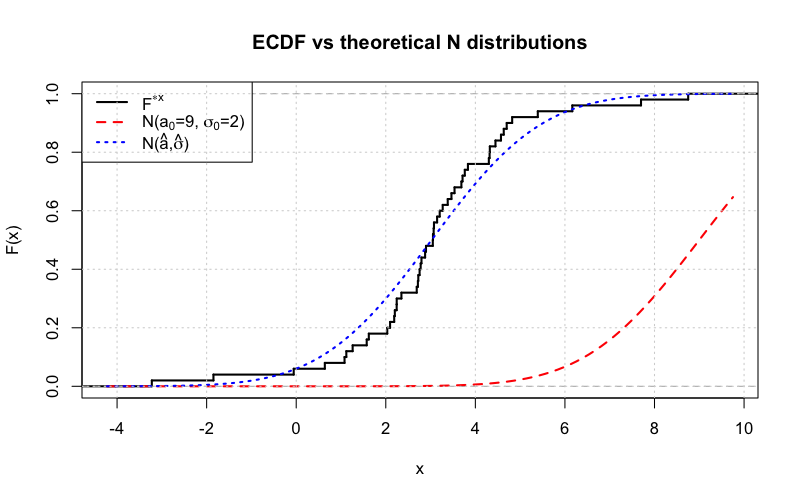
\includegraphics[width=0.7\textwidth]{plots/task2_ecdf_vs_theor}
		\caption{Задание 2: ECDF vs теоретические $N(9;\,4)$ (простая $H_0$) и $N(\hat{a},\hat\sigma^2)$ (сложная $H_0$)}
	\end{figure}
	
	\textbf{Вывод:} так как $\sqrt{n}D_n = 6{,}394 > 1{,}2238 = D_{\text{крит}}$
	(и p-value $\approx 0 < \alpha_2 = 0{,}10$), гипотеза $H_0$ \textbf{отвергается}.
	Данные не соответствуют нормальному распределению $N(9;\,4)$.
	
	%-------------------------------------------------------------
	\subsection{f) Критерий \texorpdfstring{$\chi^2$}{chi2}: простая гипотеза
		\texorpdfstring{$H_0\colon N(9;\,4)$}{}}
	
	\textbf{Задание:} используя гистограмму частот, построить критерий $\chi^2$
	проверки простой гипотезы согласия с нормальным распределением $N(9;\,4)$.
	Проверить на уровне $\alpha_2$.
	
	Границы интервалов выбраны по реальному диапазону данных так, чтобы
	наблюдения были распределены по группам. Вероятности $p_i$ вычислены
	по гипотетическому $N(9;\,4)$.
	
Минимизация через \texttt{optim}. Результат: $\hat{a}=3{,}032$, $\hat\sigma=1{,}337$.

\begin{table}[H]
	\centering
	\begin{tabular}{ccccccc}
		\toprule
		$i$ & $\mathrm{low\_b}$ & $\mathrm{up\_b}$ & $\nu_i$ & $p_i$ & $np_i$ & $\mathrm{res}^2$ \\
		\midrule
		1 & $-\infty$ & $1{,}598$ &  8 & 0{,}000107 &  0{,}005 & 11904{,}76 \\
		2 & $1{,}598$ & $2{,}721$ & 10 & 0{,}000739 &  0{,}037 &  2687{,}11 \\
		3 & $2{,}721$ & $3{,}175$ & 11 & 0{,}000947 &  0{,}047 &  2534{,}68 \\
		4 & $3{,}175$ & $4{,}067$ &  9 & 0{,}005029 &  0{,}251 &   304{,}36 \\
		5 & $4{,}067$ & $4{,}761$ &  7 & 0{,}010202 &  0{,}510 &    82{,}57 \\
		6 & $4{,}761$ & $+\infty$ &  5 & 0{,}982976 & 49{,}149 &    39{,}66 \\
		\bottomrule
		\multicolumn{6}{r}{$\chi^2 =$} & \textbf{17553{,}13} \\
	\end{tabular}
	\caption{Сводная таблица: $k=6$ интервалов по данным, простая $H_0\colon N(9;\,4)$}
\end{table}

$df=k-1=5$, $\mathrm{crit}=\chi^2_{0{,}90}(5)=9{,}236$, $p\approx 0$.

\textbf{Вывод:} $H_0\colon N(9;\,4)$ \textbf{отвергается}.
	
	%-------------------------------------------------------------
\subsection{g) Критерий \texorpdfstring{$\chi^2$}{chi2}: сложная гипотеза
	\texorpdfstring{$H_0\colon N(a,\sigma^2)$}{}}

\textbf{Задание:} построить критерий $\chi^2$ сложной гипотезы согласия
с нормальным распределением. Параметры неизвестны.

\subsubsection*{Метод проверки}

Оцениваем $a$ и $\sigma$ путём минимизации $\chi^2(a,\sigma)$:
\[
\chi^2(a,\sigma) = \sum_{j=1}^r \frac{(\nu_j - np_j(a,\sigma))^2}{np_j(a,\sigma)},
\qquad
p_j(a,\sigma) = \Phi\!\left(\frac{b_j-a}{\sigma}\right) - \Phi\!\left(\frac{b_{j-1}-a}{\sigma}\right).
\]

Минимизация через \texttt{optim}. Результат: $\hat{a}=3{,}032$, $\hat\sigma=1{,}337$.

\begin{table}[H]
	\centering
	\begin{tabular}{cccccccc}
		\toprule
		$i$ & $\mathrm{low\_b}$ & $\mathrm{up\_b}$ & $\nu_i$ & $p_i$ & $np_i$ & $\mathrm{res}$ & $\mathrm{res}^2$ \\
		\midrule
		1 & $-\infty$ & $1{,}598$ &  8 & 0{,}14167 &  7{,}083 & $+0{,}344$ & 0{,}119 \\
		2 & $1{,}598$ & $2{,}721$ & 10 & 0{,}26647 & 13{,}324 & $-0{,}911$ & 0{,}829 \\
		3 & $2{,}721$ & $3{,}175$ & 11 & 0{,}13438 &  6{,}719 & $+1{,}651$ & 2{,}727 \\
		4 & $3{,}175$ & $4{,}067$ &  9 & 0{,}23807 & 11{,}904 & $-0{,}842$ & 0{,}708 \\
		5 & $4{,}067$ & $4{,}761$ &  7 & 0{,}12137 &  6{,}068 & $+0{,}378$ & 0{,}143 \\
		6 & $4{,}761$ & $+\infty$ &  5 & 0{,}09804 &  4{,}902 & $+0{,}044$ & 0{,}002 \\
		\bottomrule
		\multicolumn{7}{r}{$\chi^2_{\min} =$} & \textbf{4{,}528} \\
	\end{tabular}
	\caption{Сводная таблица: $k=6$ интервалов, сложная $H_0\colon N(\hat{a},\hat\sigma^2)$}
\end{table}

$df = k-1-2 = 6-1-2 = 3$, $\mathrm{crit}=\chi^2_{0{,}90}(3)=6{,}251$, $p=0{,}210$.

\textbf{Вывод:} $\chi^2=4{,}528 < 6{,}251$, $H_0$ \textbf{не отвергается}.
Данные совместимы с нормальным распределением $N(3{,}032;\,1{,}788)$.
	
	\begin{figure}[H]
		\centering
		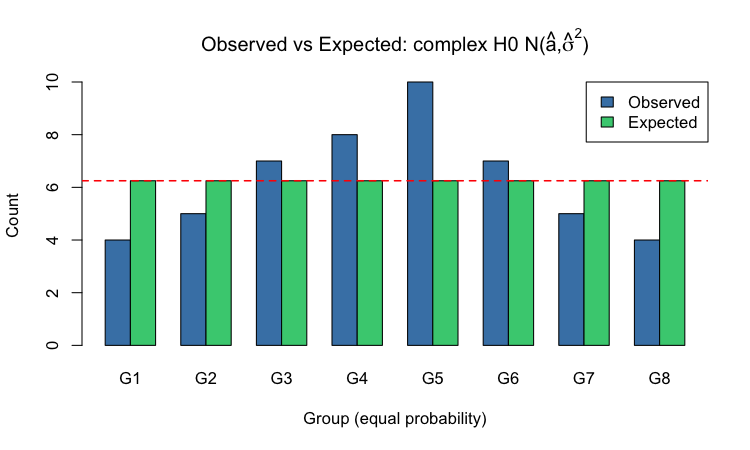
\includegraphics[width=0.48\textwidth]{plots/task2_chi2_complex}
		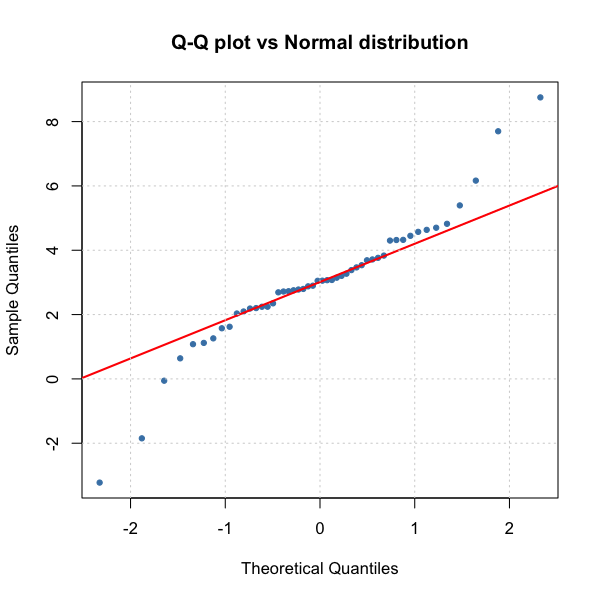
\includegraphics[width=0.48\textwidth]{plots/task2_qqplot}
		\caption{Задание 2: Наблюдаемые и ожидаемые частоты для сложной $H_0$ (слева); график квантиль-квантиль vs нормальное (справа)}
	\end{figure}
	
	%-------------------------------------------------------------
	\subsection{h) НМК Неймана--Пирсона}
	
	\textbf{Задание:} построить наиболее мощный критерий проверки простой
	гипотезы нормальности $(a,\sigma^2)=(a_0,\sigma_0^2)$ при альтернативе
	$(a,\sigma^2)=(a_1,\sigma_1^2)$. Что получится при перестановке гипотез?
	
	\subsubsection*{Постановка задачи}
	
	$H_0\colon N(9;\,4)$,\; $H_A\colon N(3;\,4)$, уровень $\alpha_2=0{,}10$.
	
	\subsubsection*{Функция правдоподобия}
	
	\[
	L(X;a,\sigma^2) = \prod_{i=1}^n \frac{1}{\sqrt{2\pi\sigma^2}}
	\exp\!\left(-\frac{(X_i-a)^2}{2\sigma^2}\right).
	\]
	
	Отношение правдоподобий ($\sigma_0=\sigma_1=2$):
	\[
	LR(X) = \exp\!\left(\frac{n(a_1-a_0)}{\sigma^2}\left(\bar{X}-\frac{a_0+a_1}{2}\right)\right).
	\]
	
	Так как $a_1-a_0 = 3-9 = -6 < 0$, то $LR(X)$ \textbf{убывает} с ростом $\bar{X}$.
	Критическая область: $\bar{X} < C$.
	
	\subsubsection*{Нахождение границы $C$}
	
	При $H_0$: $\bar{X}\sim N\!\left(9,\, \dfrac{4}{50}\right)$.
	\[
	C = a_0 + z_{1-\alpha_2}\cdot\frac{\sigma_0}{\sqrt{n}}
	= 9 - 1{,}2816\cdot\frac{2}{\sqrt{50}} = 8{,}638.
	\]
	
	\subsubsection*{Формальная запись критерия}
	
	\[
	\phi(X) = \begin{cases}
		1, & \text{если } \bar{X} < 8{,}638,\\
		0, & \text{если } \bar{X} \ge 8{,}638.
	\end{cases}
	\]
	
	\subsubsection*{Проверка гипотезы}
	
	$\bar{X}_{\text{набл}} = 3{,}023 < 8{,}638 = C$ $\Rightarrow$ $H_0$ \textbf{отвергается}.
	Мощность $\approx 1{,}0$.
	
	\subsubsection*{Смена гипотез местами}
	
	$H_0\colon N(3;\,4)$ против $H_A\colon N(9;\,4)$. Критическая область правосторонняя:
	\[
	C' = a_1 + z_{1-\alpha_2}\cdot\frac{\sigma_1}{\sqrt{n}}
	= 3 + 1{,}2816\cdot\frac{2}{\sqrt{50}} = 3{,}362.
	\]
	\[
	\phi(X) = \begin{cases}
		1, & \text{если } \bar{X} > 3{,}362,\\
		0, & \text{если } \bar{X} \le 3{,}362.
	\end{cases}
	\]
	$\bar{X}_{\text{набл}} = 3{,}023 < 3{,}362 = C'$ $\Rightarrow$ $H_0\colon N(3;\,4)$
	\textbf{не отвергается}.
	
	%-------------------------------------------------------------
	\subsection{i) Распределение Лапласа}
	
	\textbf{Задание:} в пунктах (c)--(h) заменить семейство нормальных распределений
	на двухпараметрическое семейство Лапласа:
	\[
	f(x) = \frac{1}{\sqrt{2}\,\sigma}\exp\!\left(-\frac{\sqrt{2}}{\sigma}|x-a|\right).
	\]
	
	\subsubsection*{(c) Оценки МПП}
	$\hat{a}_{\text{Lap}} = \mathrm{Me} = 3{,}052$,\;
	$\hat\sigma_{\text{Lap}} = \sqrt{2}\cdot\dfrac{1}{n}\sum|x_i-\hat{a}| = 1{,}853$.
	Смещение $\hat{a}$: $0$; $\hat\sigma$: асимптотически несмещённая.
	
	\subsubsection*{(d) ДИ для $a$}
	\[
	a \in [2{,}621;\; 3{,}483].
	\]
	
	\subsubsection*{(e) Критерий Колмогорова: $H_0\colon\mathrm{Laplace}(9;\,2)$}
	$\sqrt{n}D_n = 6{,}371 \gg 1{,}2238$. $H_0$ \textbf{отвергается}.
	
	\subsubsection*{(f) $\chi^2$ простая $H_0\colon\mathrm{Laplace}(9;\,2)$}
	$\chi^2 = 2703{,}6$, $df=6$. $H_0$ \textbf{отвергается}.
	
	\subsubsection*{(g) $\chi^2$ сложная $H_0\colon\mathrm{Laplace}(\hat{a},\hat\sigma)$}
	$\chi^2 = 8{,}199$, $df=7$, $\mathrm{crit}=12{,}017$, $p=0{,}315$.
	$H_0$ \textbf{не отвергается}.
	
	\subsubsection*{(h) НМК: $H_0\colon\mathrm{Laplace}(9;\,2)$
		vs $H_1\colon\mathrm{Laplace}(3;\,2)$}
	$\ln\Lambda = 164{,}92$, bootstrap $c\approx-166{,}0$. $H_0$ \textbf{отвергается}.
	При перестановке: $\ln\Lambda' = -164{,}92$, $H_0\colon\mathrm{Laplace}(3;\,2)$
	\textbf{не отвергается}.
	
	%=============================================================
	\newpage
	\section{Сводная таблица результатов}
	%=============================================================
	
	\begin{table}[H]
		\centering
		\renewcommand{\arraystretch}{1.3}
		\begin{tabular}{clcc}
			\toprule
			\textbf{Пункт} & \textbf{Критерий} & \textbf{Зад.\,1} & \textbf{Зад.\,2} \\
			\midrule
			b & $\xbar$ & $0{,}70$ & $3{,}023$ \\
			& $s^2$   & $0{,}541$ & $3{,}857$ \\
			& $A_s$   & $+0{,}840$ & $-0{,}184$ \\
			& $E_x$   & $0{,}398$ & $2{,}581$ \\
			\midrule
			c & МПП     & $\hat\lambda=0{,}70$ & $\hat{a}=3{,}023,\;\hat\sigma^2=3{,}779$ \\
			& Смещение & $0$ & $0$ и $-\sigma^2/n\approx-0{,}076$ \\
			\midrule
			d & ДИ      & $[0{,}468;\;0{,}932]$ & $a:[2{,}557;\;3{,}489]$ \\
			&         &                        & $\sigma^2:[2{,}849;\;5{,}569]$ \\
			\midrule
			e & Простая $H_0$ & $\chi^2=19{,}06$, откл. & Колм.\,$K_n=6{,}39$, откл. \\
			\midrule
			f & $\chi^2$ прост. & Geom: откл. & $\chi^2=288537$, откл. \\
			& $\chi^2$ слож.  & Poiss: не откл. & $\chi^2=5{,}04$, не откл. \\
			\midrule
			g & НМК & $T=35\le57$, откл. & $\bar{X}=3{,}02<C=8{,}64$, откл. \\
			& Перестановка & $T=35<45$, не откл. & $\bar{X}=3{,}02<C'=3{,}36$, не откл. \\
			\bottomrule
		\end{tabular}
		\caption{Сводка основных результатов ($\alpha_1=0{,}05$, $\alpha_2=0{,}10$)}
	\end{table}
	
	\end{document}
	